%
%--------------------------------------------------------

%  Challenge Problem 1 
%  Shantanu Yadav, EE20MTech12001
%  IIT Hyderabad
%--------------------------------------------------------
%
\documentclass[12pt]{article}
\usepackage{graphicx}
\usepackage{amsmath}

\begin{document}
\begin{center}
	{\Large \bf IIT Hyderabad} \\ \vspace{2ex}
	{\large \bf SHANTANU YADAV, EE20MTECH12001 }\\
	\vspace{2ex}
	{\large \bf CHALLENGE PROBLEM 1} \\
\end{center}
	\hrule

\vspace{2ex}
\begin{center}
{\underline{\Large \bf Lines and Planes}}
\end{center}

\section*{Problem Statement}


\section*{Shortest distance between two skew lines}
	Let the two lines are $l_1$ and $l_2$. The equations of these lines are
\begin{align*}
\overrightarrow{r} = \overrightarrow{a_1} + \lambda \overrightarrow{b_1}
\hspace{2ex} \text{and} \hspace{2ex} 
\overrightarrow{r} = \overrightarrow{a_2} + \mu \overrightarrow{b_2}
\hspace{2ex} \text{respectively.}
\end{align*}
These lines pass through the points $A$ and $B$ whose position vectors are
$\overrightarrow{a_1}$ and  $\overrightarrow{a_2}$.
Let us assume that the lines are parallel to the vectors 
$\overrightarrow{b_1}$ and  $\overrightarrow{b_2}$ respectively.

\begin{figure}[htbp]
	\centering
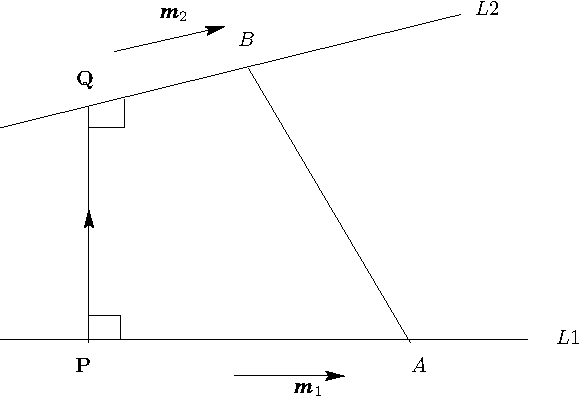
\includegraphics[width=0.5\linewidth]{skewlines.png}
\end{figure}

\noindent
Let $\overrightarrow{PQ}$ be the shortest distance vector between $l_1$ and
$l_2$. Then $\overrightarrow{PQ}$ is perpendicular to both
$l_1$ and $l_2$ which are parallel to
$\overrightarrow{b_1}$ and  $\overrightarrow{b_2}$ respectively.
Therefore, $\overrightarrow{PQ}$ is perpendicular to both
$\overrightarrow{b_1}$ and  $\overrightarrow{b_2}$. 
But $\overrightarrow{b_1} \times \overrightarrow{b_2}$ is perpendicular to both
$\overrightarrow{b_1}$ and  $\overrightarrow{b_2}$. 
Therefore, $\overrightarrow{PQ}$ is parallel to
$\overrightarrow{b_1} \times \overrightarrow{b_2}$.
\\

\noindent
Let $\hat{n}$ is a unit vector along $\overrightarrow{PQ}$. Then, we have
\begin{align*}
\hat{n} =\pm \frac{ \overrightarrow{b_1} \times \overrightarrow{b_2} }{
|\overrightarrow{b_1} \times \overrightarrow{b_2}| }
\end{align*}
therefore, \hfill $PQ =$ projection of $\overrightarrow{AB}$ on
	$\overrightarrow{PQ}$  \hfill ~\\

\noindent
$\implies$ \hfill $PQ =\overrightarrow{AB} \cdot \hat{n}$ \hfill ~\\
\begin{align}
PQ &= \pm ( \overrightarrow{a_2} - \overrightarrow{a_1}) \cdot
\left\{ \frac{ \overrightarrow{b_1} \times \overrightarrow{b_2} }{
	|\overrightarrow{b_1} \times \overrightarrow{b_2}| } \right\} \\
   &= \pm 
	\frac{ (\overrightarrow{b_1} \times \overrightarrow{b_2} ) \cdot
	( \overrightarrow{a_2} - \overrightarrow{a_1}) }{
	|\overrightarrow{b_1} \times \overrightarrow{b_2}| }  \nonumber
\end{align}
Since the distance $PQ$ is to be taken as positive, hence
\begin{align}
PQ = \left| \frac{ (\overrightarrow{b_1} \times \overrightarrow{b_2} ) \cdot
	( \overrightarrow{a_2} - \overrightarrow{a_1}) }{
	|\overrightarrow{b_1} \times \overrightarrow{b_2}| } \right|
\end{align}

\end{document}
